\documentclass[11pt,a4paper]{article}

\usepackage[utf8]{inputenc}
\usepackage[T1]{fontenc}
\usepackage{amsmath,amssymb}
\usepackage{booktabs}
\usepackage{graphicx}
\usepackage{hyperref}
\usepackage[margin=2.5cm]{geometry}
\usepackage{algorithm}
\usepackage{algorithmic}
\usepackage{xcolor}
\usepackage{enumitem}

\definecolor{accent}{RGB}{37,99,235}

\title{\textbf{Consensus Multi-Layer Edge Combination\\for Scientific Paper Clustering}}
\author{Young Jin Kim}
\date{April 2026}

\begin{document}
\maketitle

\begin{abstract}
We propose a multi-layer edge combination pipeline for CPM Leiden clustering of scientific paper networks. The pipeline combines citation-based edges (direct citation, bibliographic coupling, co-citation) with embedding-based edges using a \emph{consensus} strategy: edges confirmed by multiple independent layers receive multiplicative weight amplification. Combined with per-node top-$k$ filtering, $1/\text{rank}$ normalization, and automatic resolution ($\gamma$) selection, the pipeline produces balanced cluster distributions across fields with varying citation densities. Experiments on two OpenAlex fields (Chemical Engineering, 115K papers; Arts \& Humanities, 754K papers) demonstrate that (1) consensus combination assigns boundary nodes more accurately than simple summation (29:26 in 55 LLM blind reviews), (2) adding embedding edges reduces cluster count by 60\% while doubling average cluster size, and (3) automatic $\gamma$ search is essential as optimal resolution shifts 24--32$\times$ between 3-layer and 4-layer configurations.
\end{abstract}

%% ─────────────────────────────────────────────────────────
\section{Introduction}

Clustering scientific papers into research communities requires constructing a similarity network from multiple heterogeneous signals. Citation-based measures---direct citation (DC), bibliographic coupling (BC), and co-citation (CC)---capture different aspects of scholarly relatedness but have uneven coverage: BC may cover only 49\% of papers in humanities fields, while DC is universally available but sparse. Embedding-based similarity (e.g., SPECTER2 $k$-NN) provides universal coverage but may introduce noise from stylistic rather than topical similarity.

The central question is: \emph{how should these heterogeneous layers be combined into a single network for community detection?}

We address three sub-problems:
\begin{enumerate}[nosep]
    \item \textbf{Normalization}: Edge weights across layers have incomparable scales.
    \item \textbf{Combination}: How to merge normalized layers into one edge table.
    \item \textbf{Resolution}: The CPM resolution parameter $\gamma$ must adapt to the combined network's density.
\end{enumerate}

%% ─────────────────────────────────────────────────────────
\section{Method}

\subsection{Pipeline Overview}

\begin{algorithm}[h]
\caption{Consensus Multi-Layer Combination}
\begin{algorithmic}[1]
\REQUIRE Edge tables $\{E_\ell\}_{\ell=1}^{L}$ for $L$ layers, target $\text{max}_\%$
\FOR{each layer $\ell$}
    \STATE $E_\ell' \leftarrow \textsc{TopK}(E_\ell, k{=}30)$ \COMMENT{per-node top-$k$ filter}
    \STATE $E_\ell'' \leftarrow \textsc{RankNorm}(E_\ell')$ \COMMENT{$w_{ij} \leftarrow 1/\text{rank}(w_{ij})$}
\ENDFOR
\STATE $E_{\text{combined}} \leftarrow \textsc{ConsensusSum}(\{E_\ell''\})$ \COMMENT{Eq.~\ref{eq:consensus}}
\STATE $E_{\text{gcc}} \leftarrow \textsc{GCC}(E_{\text{combined}})$ \COMMENT{giant connected component}
\STATE $\gamma^* \leftarrow \textsc{AutoGamma}(E_{\text{gcc}}, \text{max}_\%)$ \COMMENT{binary search}
\STATE $\mathcal{C} \leftarrow \textsc{Leiden}(E_{\text{gcc}}, \gamma^*)$
\STATE $\mathcal{C}' \leftarrow \textsc{Postprocess}(\mathcal{C})$ \COMMENT{cascade + Dijkstra}
\RETURN $\mathcal{C}'$
\end{algorithmic}
\end{algorithm}

\subsection{Top-$k$ Filtering (Step 1)}

Each layer independently retains only the $k$ strongest neighbors per node (symmetric mode: edge kept if \emph{either} endpoint has it in their top-$k$). This removes long-tail noise that otherwise dominates after normalization. With $k{=}30$, cross-cluster edges drop from 70\% to 31\% of the combined network.

\subsection{$1/\text{rank}$ Normalization (Step 2)}

Within each filtered layer, edges are sorted by weight descending and assigned $w_{ij} \leftarrow 1/\text{rank}(w_{ij})$. This is scale-free: it preserves only the ordering, making heterogeneous layers (BC cosine similarity vs. DC fractional counts vs. Emb $k$-NN distance) directly comparable.

\subsection{Consensus Sum (Step 3)}

\begin{equation}\label{eq:consensus}
    w_{ij}^{\text{cons}} = \left(\sum_{\ell=1}^{L} w_{ij}^{(\ell)}\right) \times n_{ij}
\end{equation}

where $n_{ij} = |\{\ell : (i,j) \in E_\ell'\}|$ is the number of layers containing edge $(i,j)$ after top-$k$ filtering. Edges confirmed by multiple independent signals receive multiplicative amplification.

\paragraph{Rationale.} In a 3-layer (BC+CC+DC) configuration:
\begin{itemize}[nosep]
    \item 73\% of edges appear in only 1 layer ($n_{ij}{=}1$, no boost)
    \item 21\% appear in 2 layers ($n_{ij}{=}2$, $2\times$ boost)
    \item 6\% appear in all 3 layers ($n_{ij}{=}3$, $3\times$ boost)
\end{itemize}
The 6\% of 3-layer edges form \emph{cluster cores} in Leiden, while single-layer edges become relatively weak, preventing mega-cluster absorption.

\subsection{Automatic Resolution Selection (Step 4)}

Adding layers changes the effective edge density, shifting optimal $\gamma$ non-linearly. We observe 24--32$\times$ shifts between 3-layer and 4-layer configurations---unpredictable from edge count ratios alone (4.2$\times$). We therefore use binary search on log-scale $\gamma$ to find the resolution where the largest cluster is $<\text{max}_\%$ of total nodes (default 3\%).

%% ─────────────────────────────────────────────────────────
\section{Experimental Setup}

\subsection{Data}

Two OpenAlex fields with contrasting citation densities:

\begin{table}[h]
\centering
\caption{Dataset characteristics (top-30 filtered)}
\begin{tabular}{lrrrr}
\toprule
 & \multicolumn{2}{c}{Field 15 (Chem. Eng.)} & \multicolumn{2}{c}{Field 12 (Arts \& Hum.)} \\
Layer & Edges & Coverage & Edges & Coverage \\
\midrule
BC cosine & 1.56M & 86\% & -- & 49\% \\
CC cosine & 524K & 46\% & -- & 18\% \\
DC fractional & 808K & 100\% & -- & 100\% \\
Emb $k$-NN & 2.86M & 100\% & 19.3M & 100\% \\
\midrule
DC avg degree & \multicolumn{2}{c}{16} & \multicolumn{2}{c}{5} \\
Emb avg degree & \multicolumn{2}{c}{50} & \multicolumn{2}{c}{51} \\
\bottomrule
\end{tabular}
\end{table}

\subsection{Comparison Methods}

\paragraph{Normalization:} raw, $1/\text{rank}$, quantile.
\paragraph{Combination:} sum ($\sum w$), max ($\max w$), vote (count), consensus ($\sum w \times n$).

\subsection{Evaluation}

\begin{enumerate}[nosep]
    \item \textbf{Structural}: cluster count, max cluster \%, size distribution balance.
    \item \textbf{LLM blind review} (GPT-4o-mini, 55 cases): three criteria on disagreement nodes between sum and consensus:
    \begin{itemize}[nosep]
        \item \emph{Belonging}: ``Which group does this paper naturally belong to?''
        \item \emph{Group cohesion}: independent quality score per cluster (1--5).
        \item \emph{Outlier count}: papers that don't fit in the cluster.
    \end{itemize}
\end{enumerate}

%% ─────────────────────────────────────────────────────────
\section{Results}

\subsection{Normalization $\times$ Combination Grid}

\begin{table}[h]
\centering
\caption{Field 15, $\gamma{=}10^{-6}$, min\_size$=$100, top-30, GCC. Cluster count and max cluster \%.}
\begin{tabular}{llrr}
\toprule
Normalization & Combination & Clusters & Max \% \\
\midrule
raw & sum & 189 & 12.2 \\
raw & vote & 149 & 15.5 \\
\textbf{1/rank} & \textbf{sum} & \textbf{282} & \textbf{2.4} \\
\textbf{1/rank} & \textbf{consensus} & \textbf{298} & \textbf{2.5} \\
1/rank & vote & 149 & 16.5 \\
quantile & sum & 156 & 15.8 \\
\bottomrule
\end{tabular}
\end{table}

$1/\text{rank}$ with sum or consensus produces the most balanced distributions. Vote is invariant to normalization (binary). Raw sum creates dominant clusters.

\subsection{Sum vs. Consensus: LLM Evaluation}

\begin{table}[h]
\centering
\caption{Triple evaluation on disagreement nodes ($\gamma{=}10^{-4}$, Field 15).}
\begin{tabular}{lccc}
\toprule
Criterion & Sum & Consensus & Better \\
\midrule
Belonging (wins, $n{=}55$) & 26 & \textbf{29} & Consensus \\
Cohesion (avg, 1--5) & 4.4 & 4.4 & Tie \\
Outliers (avg per 8 neighbors) & 1.3 & 1.3 & Tie \\
\bottomrule
\end{tabular}
\end{table}

Consensus assigns boundary nodes more accurately. Internal cluster quality is equivalent.

\paragraph{By cluster size bucket (30 cases):}
\begin{itemize}[nosep]
    \item \textbf{Large ($>$500)}: Sum 7:3 --- sum's mega-clusters win by volume.
    \item \textbf{Medium (200--500)}: Consensus 6:4 --- consensus correctly separates.
    \item \textbf{Small ($<$200)}: Tie 5:5.
\end{itemize}

\subsection{3-Layer vs. 4-Layer (+Embedding)}

\begin{table}[h]
\centering
\caption{Auto-gamma results (target max $< 3\%$).}
\begin{tabular}{lrrrr}
\toprule
Config & Auto $\gamma$ & Clusters & Max \% & Avg size \\
\midrule
Field 15, 3L & $5.62 \times 10^{-5}$ & 251 & 3.0 & 459 \\
Field 15, 4L & $1.33 \times 10^{-3}$ & 221 & 2.8 & 521 \\
\midrule
Field 12, 3L & $1.78 \times 10^{-6}$ & 1{,}157 & 2.9 & 651 \\
\textbf{Field 12, 4L} & $\mathbf{5.62 \times 10^{-5}}$ & \textbf{445} & \textbf{2.9} & \textbf{1{,}693} \\
\bottomrule
\end{tabular}
\end{table}

Adding embedding edges consistently improves partitioning:
\begin{itemize}[nosep]
    \item Field 15: 12\% fewer clusters, 13\% larger avg size.
    \item Field 12: \textbf{62\% fewer clusters, 160\% larger avg size} --- embedding fills citation gaps in humanities.
\end{itemize}

The $\gamma$ ratio between 3L and 4L is 24$\times$ (Field 15) to 32$\times$ (Field 12), confirming that automatic search is essential.

\subsection{Consensus Mechanism Analysis}

The consensus/sum weight ratio is exactly $n_{ij} \in \{1, 2, 3, 4\}$:

\begin{table}[h]
\centering
\caption{Edge distribution by layer count (Field 15, 3-layer).}
\begin{tabular}{crrl}
\toprule
$n_{ij}$ & Fraction & Boost & Role \\
\midrule
1 & 73\% & $1\times$ & Boundary/noise \\
2 & 21\% & $2\times$ & Supporting \\
3 & 6.5\% & $3\times$ & \textbf{Cluster cores} \\
\bottomrule
\end{tabular}
\end{table}

The 6.5\% of 3-layer edges, amplified to $3\times$ weight, dominate Leiden's objective function and form cluster nuclei. Single-layer edges become relatively weak, preventing the mega-cluster absorption observed with simple summation.

\subsection{Temporal Edge Landscape}

Each layer exhibits a distinct temporal pattern, visible in the year$\times$year edge density heatmaps (Figure~\ref{fig:landscape}).

\begin{figure}[h]
\centering
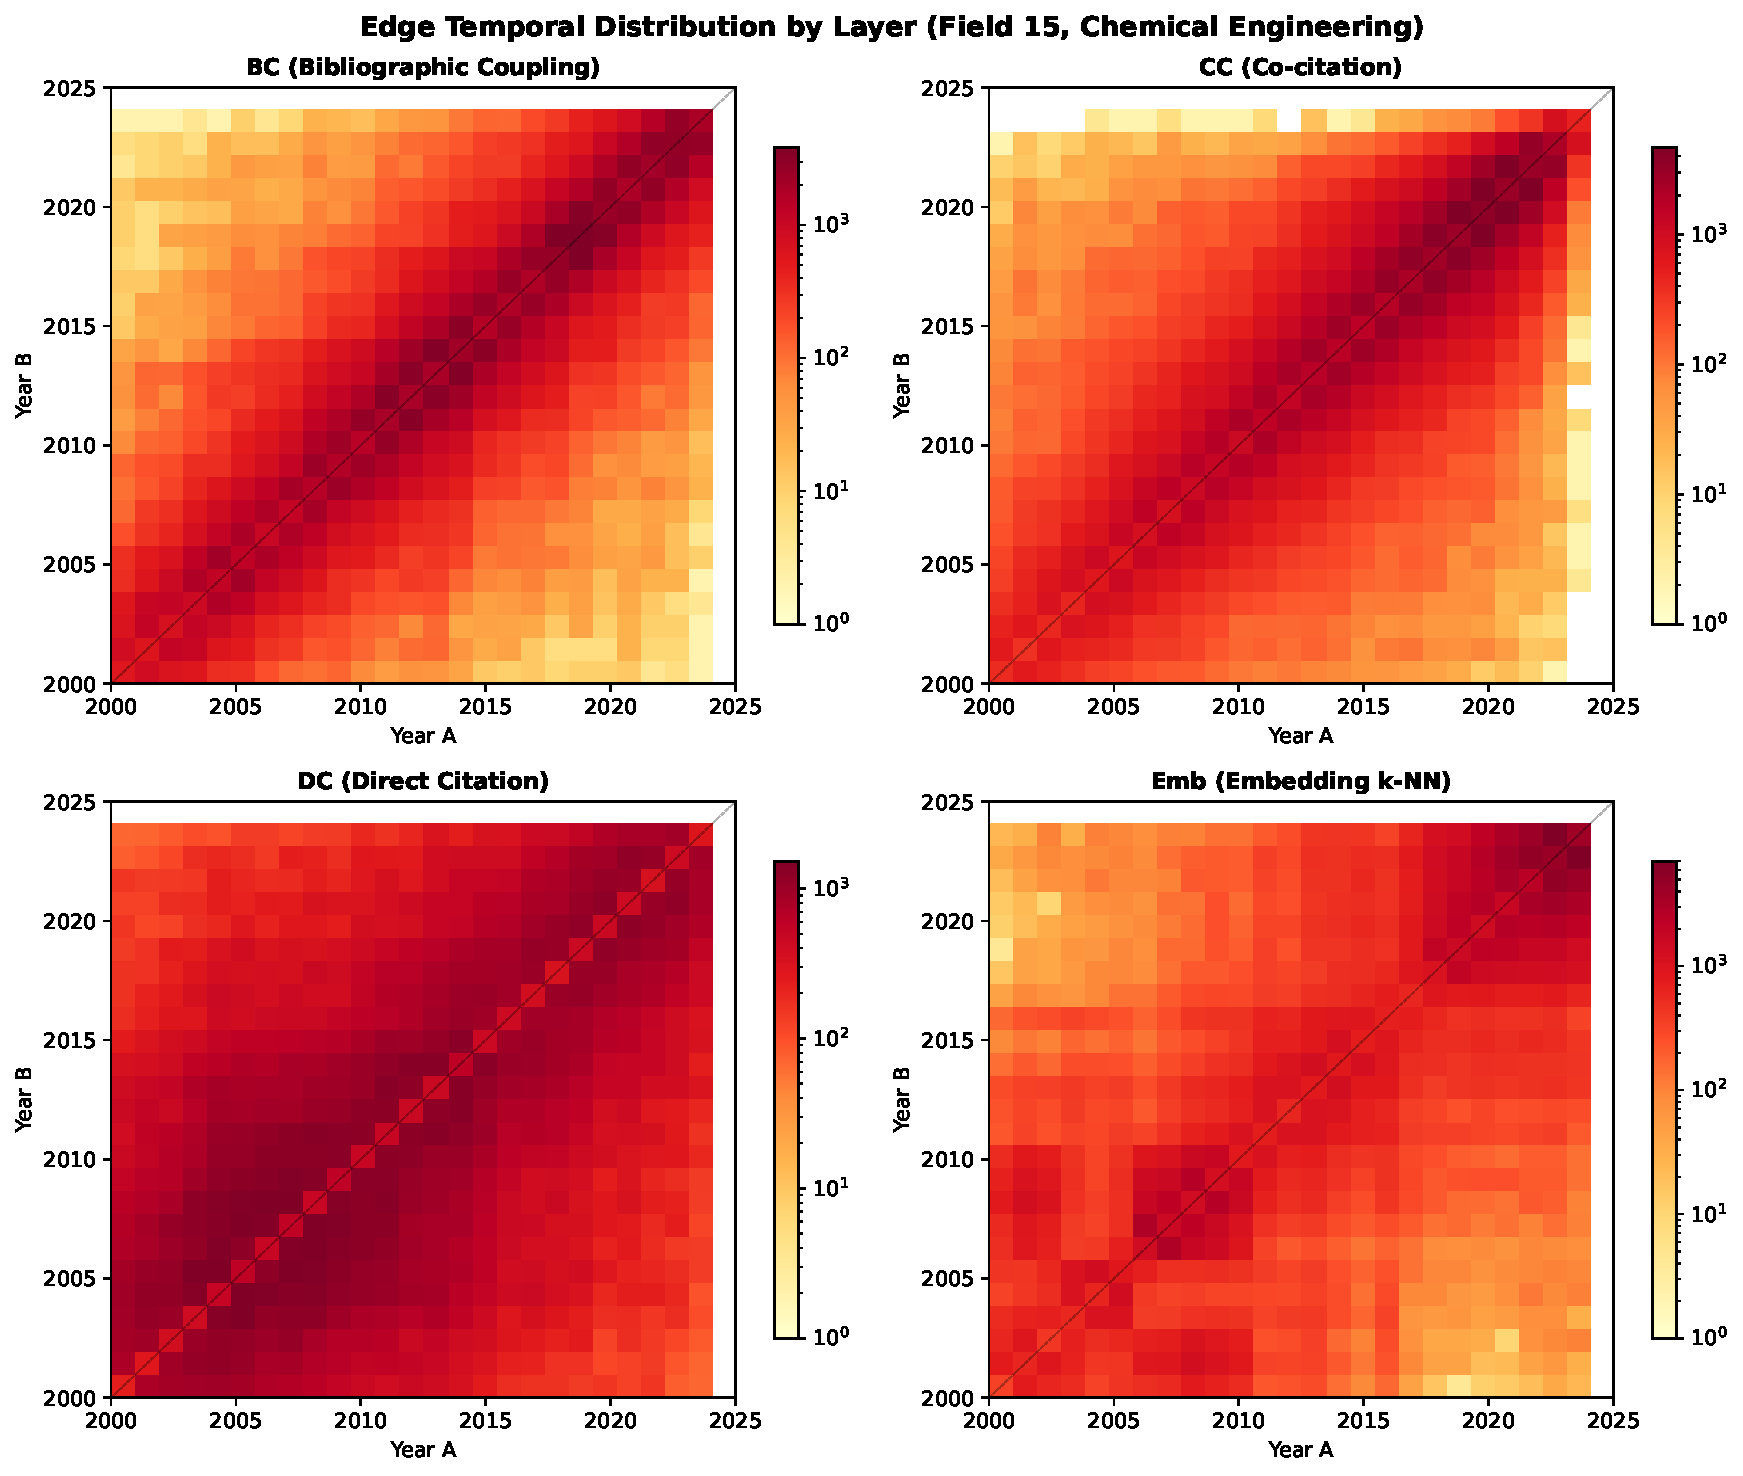
\includegraphics[width=\textwidth]{figures/edge_landscape_f15.pdf}
\caption{Year$\times$year edge density (log scale) for four layers in Field~15. BC concentrates on the diagonal (same-era papers); DC spreads widely (citing past); CC lies between; Emb shows moderate diagonal concentration.}
\label{fig:landscape}
\end{figure}

\begin{table}[h]
\centering
\caption{Temporal concentration: fraction of edges within $\pm$3 years of the diagonal.}
\begin{tabular}{lrrl}
\toprule
Layer & Diagonal $\pm$3yr & Asymmetry & Character \\
\midrule
BC & 78.0\% & 0.50 & Same-era shared references \\
CC & 73.7\% & 0.50 & Slightly broader (classic papers) \\
Emb & 62.3\% & 0.50 & Text similarity $\propto$ era \\
DC & 44.0\% & 0.50 & Widest (past citations) \\
\bottomrule
\end{tabular}
\end{table}

Stronger edges are temporally tighter: among BC edges, the top~1\% by weight have 99.4\% of connections within $\pm$3~years (Figure~\ref{fig:quantiles}).  This confirms that consensus weighting preferentially amplifies temporally coherent, topically focused connections.

\begin{figure}[h]
\centering
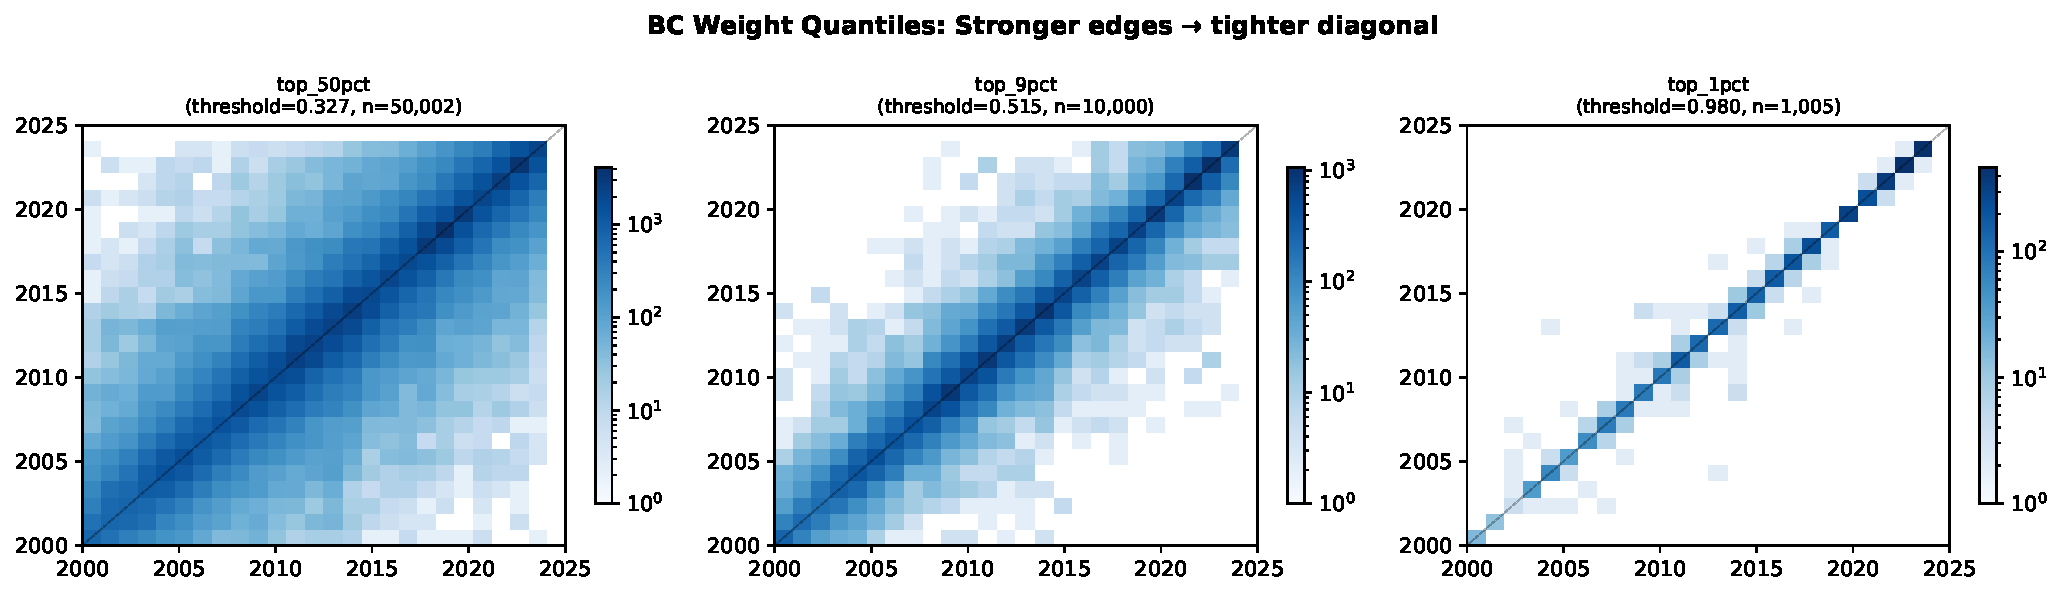
\includegraphics[width=\textwidth]{figures/bc_weight_quantiles_f15.pdf}
\caption{BC weight quantile maps: stronger edges concentrate increasingly on the diagonal. Top~1\% edges connect almost exclusively same-era papers.}
\label{fig:quantiles}
\end{figure}

\begin{figure}[h]
\centering
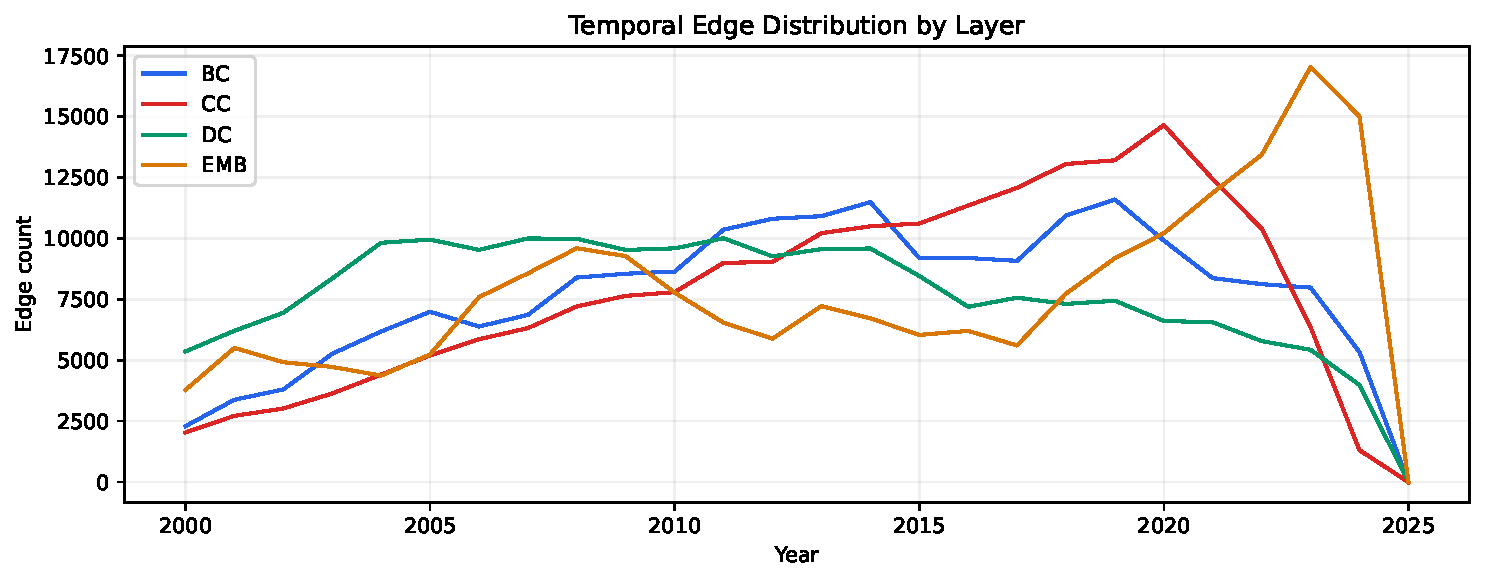
\includegraphics[width=0.8\textwidth]{figures/marginal_comparison_f15.pdf}
\caption{Temporal edge distribution (marginal) across layers. BC and CC peak in recent years; DC is flatter due to cumulative citations; Emb coverage is uniform.}
\label{fig:marginal}
\end{figure}

\subsection{Consensus Level Analysis}

Decomposing edges by consensus level reveals that higher consensus correlates with tighter temporal concentration (Figure~\ref{fig:consensus_year}).

\begin{figure}[h]
\centering
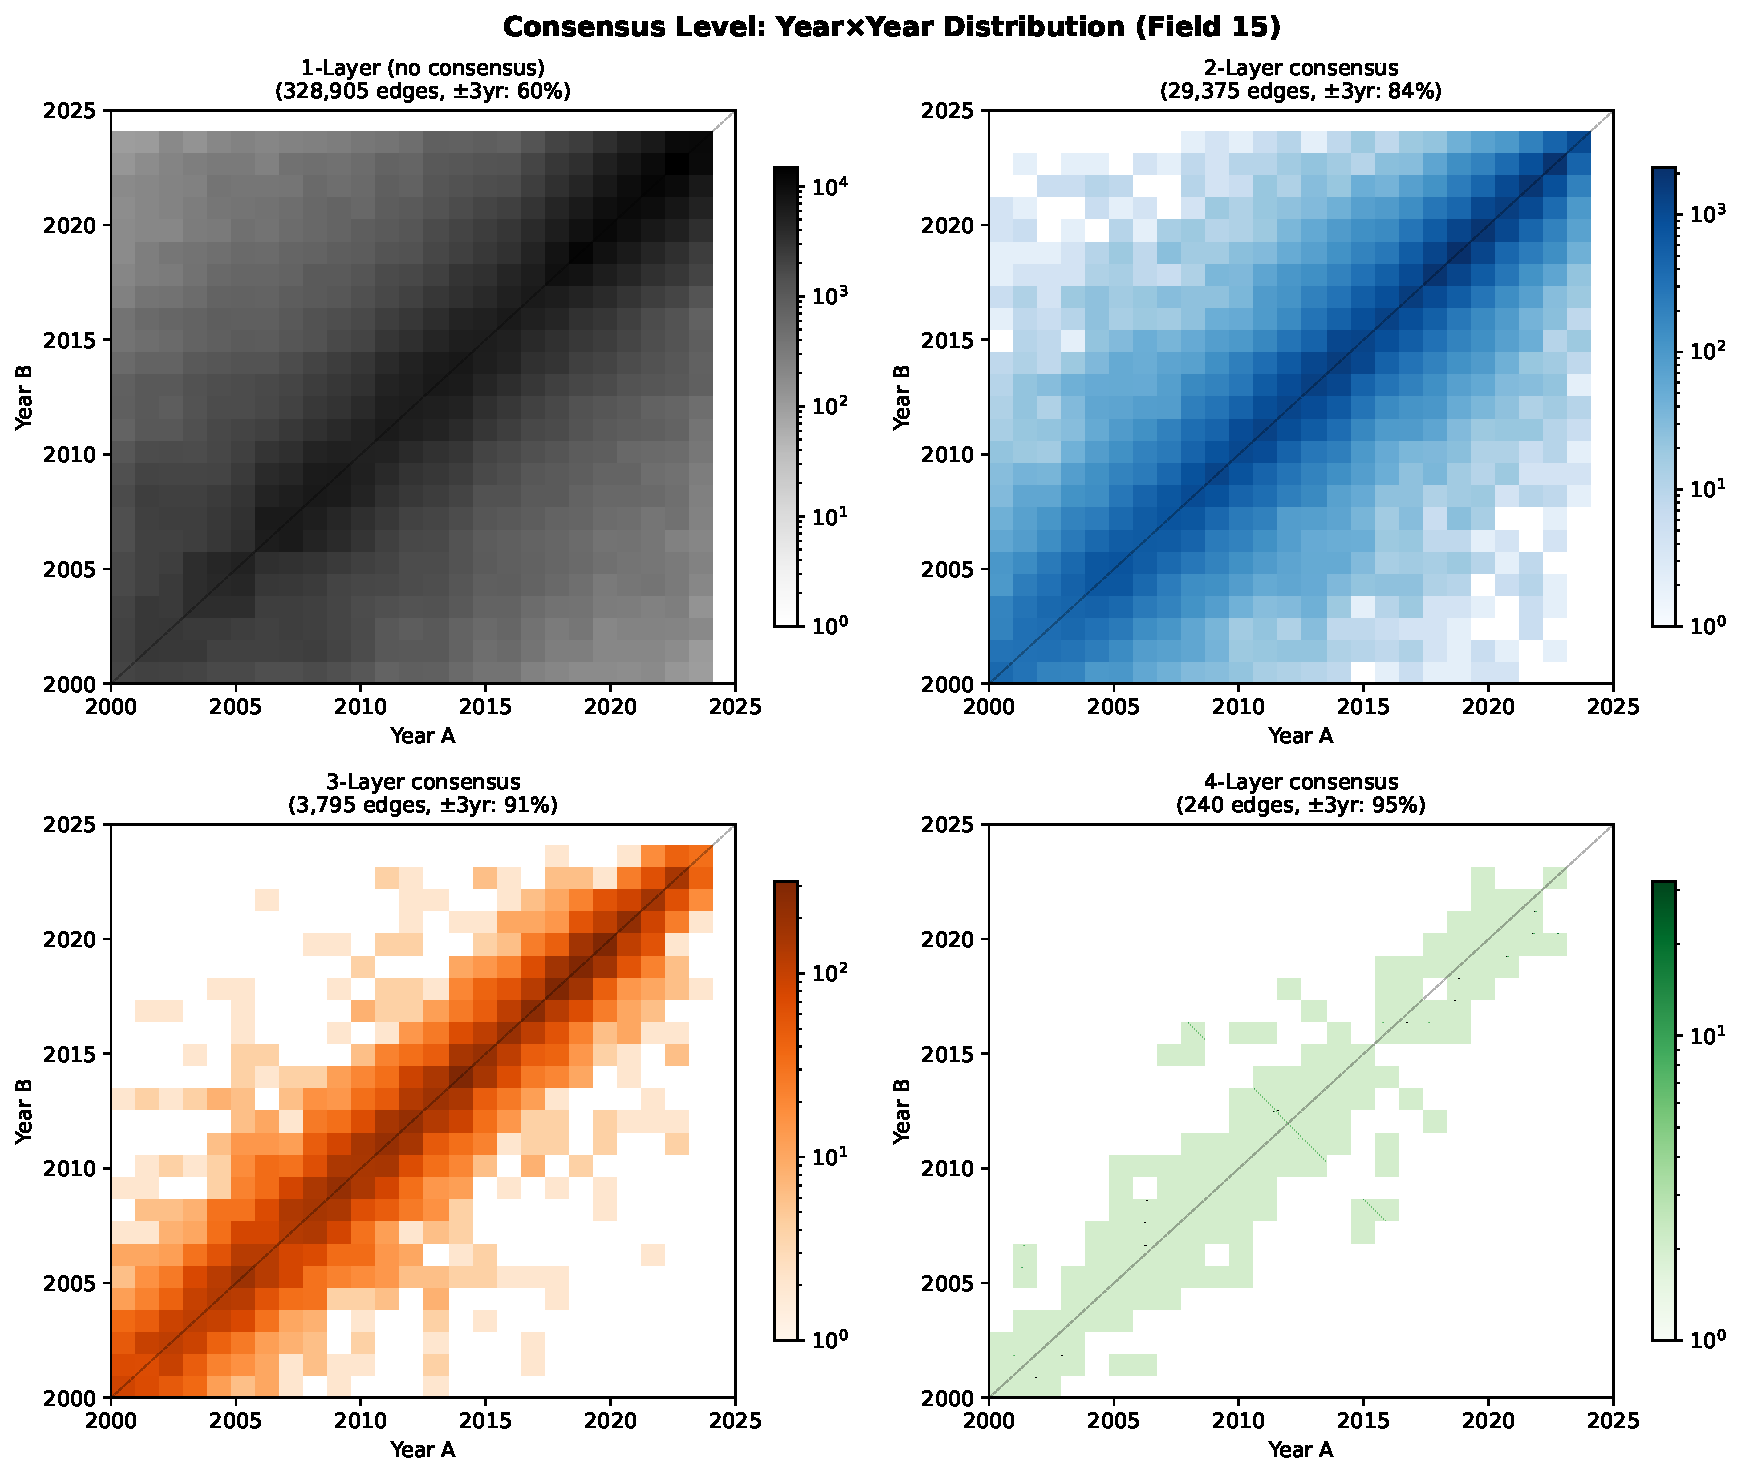
\includegraphics[width=\textwidth]{figures/consensus_levels_year_f15.pdf}
\caption{Year$\times$year heatmaps by consensus level. 1-layer edges (91\% of total) spread broadly; 3--4 layer edges concentrate sharply on the diagonal.}
\label{fig:consensus_year}
\end{figure}

\begin{table}[h]
\centering
\caption{Consensus level statistics (Field 15, 4 layers).}
\begin{tabular}{crrrrr}
\toprule
Consensus & Edges & Fraction & Diagonal $\pm$3yr & Median $w^{\text{cons}}$ \\
\midrule
1-layer & 328{,}905 & 90.8\% & 60\% & $\approx 0$ \\
2-layer & 29{,}375 & 8.1\% & 84\% & 0.0001 \\
3-layer & 3{,}795 & 1.0\% & 91\% & 0.0005 \\
4-layer & 240 & 0.1\% & 95\% & 0.0012 \\
\bottomrule
\end{tabular}
\end{table}

The consensus weight distribution and temporal profile per level are shown in Figure~\ref{fig:consensus_weight}.

\begin{figure}[h]
\centering
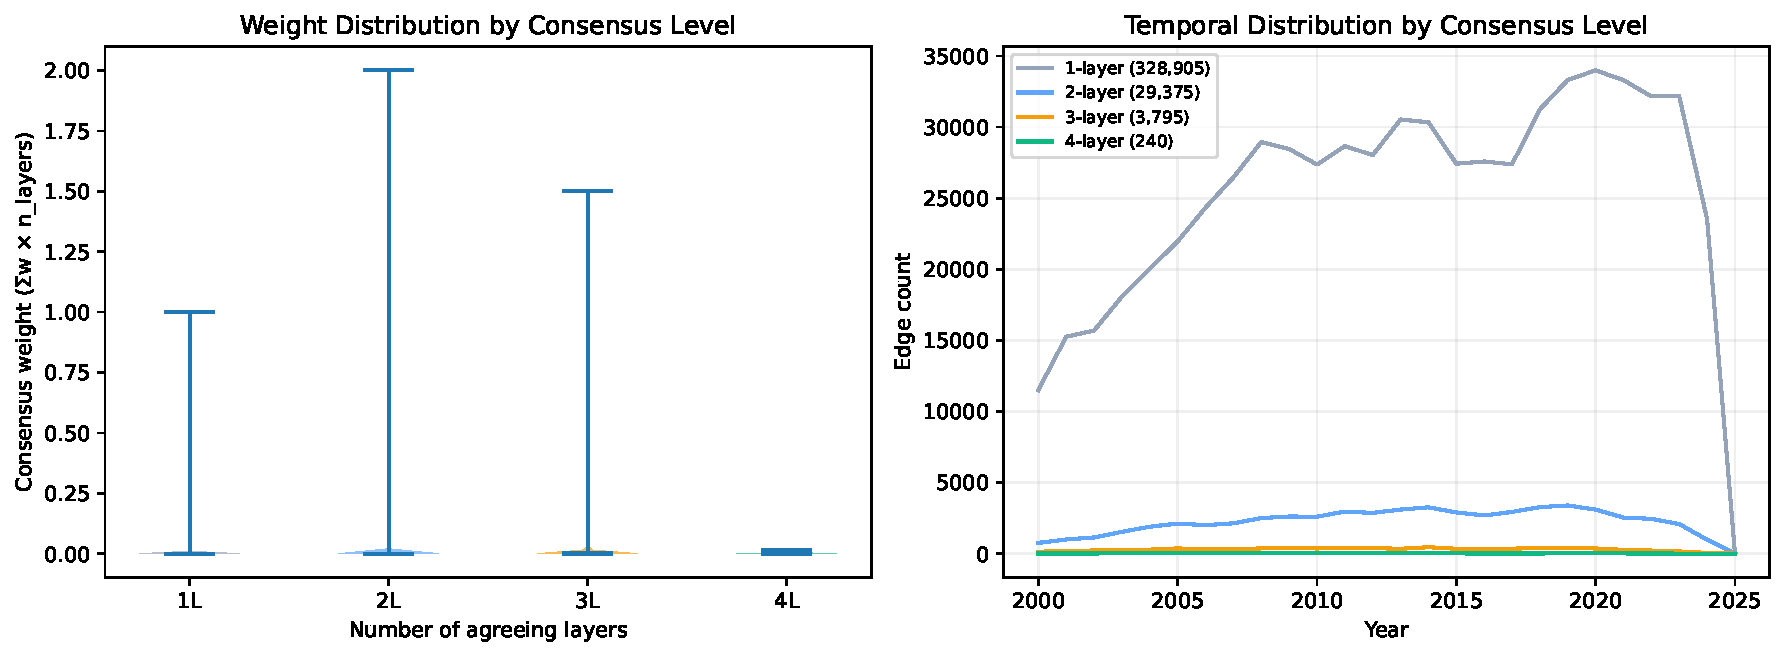
\includegraphics[width=\textwidth]{figures/consensus_weight_temporal_f15.pdf}
\caption{Left: consensus weight distribution (violin) by level---higher consensus produces heavier, more distinguishable weights. Right: temporal edge distribution per level---multi-layer edges peak in recent years where all data sources overlap.}
\label{fig:consensus_weight}
\end{figure}

This analysis confirms that consensus weighting achieves its intended effect: the small minority of multi-layer edges (9.2\%) receive disproportionate weight, forming temporally coherent cluster cores, while the single-layer majority (90.8\%) acts as supporting context.

%% ─────────────────────────────────────────────────────────
\section{Discussion}

\paragraph{Why consensus works.} CPM Leiden optimizes $H = \sum_c \left[e_c - \gamma \binom{n_c}{2}\right]$, where $e_c$ is internal edge weight. Consensus weighting amplifies edges that multiple independent measures agree on, concentrating weight in true communities. This creates a natural hierarchy: multi-layer cores attract single-layer periphery.

\paragraph{Embedding layer integration.} Embedding $k$-NN edges have universal coverage (avg degree $\approx 50$) unlike citation layers (DC avg degree $= 5$ in humanities). Na\"ively adding Emb to consensus increases $n_{ij}$ globally, collapsing the differentiation. The solution is \textbf{not} to exclude Emb but to \textbf{automatically adjust $\gamma$}: auto-gamma search absorbs the density shift, letting Emb fill citation gaps while consensus preserves cluster structure.

\paragraph{Field dependence.} Citation-poor fields (Arts \& Humanities: 3-layer overlap 0.1\%) benefit most from Emb addition (160\% avg size improvement) because citation layers alone produce excessive fragmentation. Citation-rich fields (Chemical Engineering: 3-layer overlap 2.2\%) see moderate improvement (13\%).

%% ─────────────────────────────────────────────────────────
\section{Conclusion}

We recommend the following pipeline for multi-layer scientific paper clustering:

\begin{enumerate}[nosep]
    \item \textbf{Top-30} per-node filtering on each layer.
    \item \textbf{$1/\text{rank}$} normalization for scale-free comparison.
    \item \textbf{Consensus weighting sum} $(\sum w \times n_{\text{layers}})$ for multi-layer agreement.
    \item \textbf{GCC filtering} to remove isolated components.
    \item \textbf{Auto-gamma} binary search targeting max cluster $< 3\%$.
    \item \textbf{Leiden + postprocess} with cascading $\gamma$ descent.
\end{enumerate}

This pipeline adapts automatically to varying citation densities across fields and layer configurations, producing balanced cluster distributions without manual parameter tuning.

\end{document}
